\documentclass{article}
\usepackage{amsmath}
\usepackage{graphicx}
\usepackage{float} % This package helps with figure placement
\usepackage{subcaption} % For subfigures
\usepackage[export]{adjustbox} % For additional options in \includegraphics
\usepackage{wrapfig} % For wrapping text around figures

\graphicspath{{/home/hp/nayanika/github/GPX6/figures/}} % Ensure the path is correct

\begin{document}

\title{Your Title Here}
\author{Your Name}
\date{\today}
\maketitle

\section{Results and Discussion}

Our comprehensive study on the wild type and variants demonstrates the evolution of glutathione peroxidase protein 6 cys and selenium protein. 
Despite the differences in the cysteine and selenocysteine parameters in the system, they show a wide range of associated evolutionary pathways. 
We first optimized the reaction, one step in a stepwise mechanism going from selenol to selenolate of selenocysteine and from thiol to thiolate ion in the case of cysteine, while setting up the Empirical Valence Bond Simulation. 
The substrate hydrogen peroxide was placed at the distance from selenocysteine/cysteine and glutamine83 as mentioned in the QM/MM calculations by Morokuma.

\subsection{Free Energy Changes}

Here, we present the free energy changes for the wild type and mutant systems. The table below summarizes the mean free energy values (Mean dG* and Mean dG0) for the systems we analyzed.

All the systems listed have positive dG* values, indicating that the processes are non-spontaneous under the experimental conditions. All systems exhibit negative dG0 values, suggesting that they are spontaneous under standard conditions. The variability in dG0 values among the mutant systems suggests that the specific mutations (e.g., S47A, F48Y) can significantly influence the free energy changes, potentially reflecting changes in stability or interactions within the system.

% Include the external table
\begin{table}[ht]
    \centering
    \begin{tabular}{|c|c|c|}
    \hline
    System & Mean dG* (kcal/mol) & Mean dG0 (kcal/mol) \\
    \hline
WT-Mouse Cys & 16.45 \pm 0.56 kcal/mol & -59.70 \pm 1.54 kcal/mol \ \\
    \hline
WT-Human Sec & 13.69 \pm 0.95 kcal/mol & -64.82 \pm 1.69 kcal/mol \ \\
    \hline
S47A,F48Y,T54Q,R99C & 19.34 \pm 0.58 kcal/mol & -47.63 \pm 2.85 kcal/mol \ \\
    \hline
F48Y,T52A,T54Q,R99C & 19.83 \pm 0.72 kcal/mol & -39.63 \pm 2.80 kcal/mol \ \\
    \hline
S47A,F48Y,T52A,R99C & 18.03 \pm 0.62 kcal/mol & -52.45 \pm 2.62 kcal/mol \ \\
    \hline
S47A,T52A,T54Q,R99C & 14.40 \pm 0.80 kcal/mol & -61.56 \pm 2.70 kcal/mol \ \\
    \hline
S47A,F48Y,T52A,T54Q & 17.78 \pm 0.89 kcal/mol & -57.35 \pm 2.19 kcal/mol \ \\
    \hline
Mouse Cys - S47A,F48Y,T52A,T54Q,R99C & 16.27 \pm 0.50 kcal/mol & -62.54 \pm 1.60 kcal/mol \ \\
    \hline
Mouse Sec - S47A,F48Y,T52A,T54Q,R99C & 12.21 \pm 0.62 kcal/mol & -69.17 \pm 1.64 kcal/mol \ \\
    \hline
Human Cys - A47S,Y48F,A52T,Q54T,C99R & 12.31 \pm 0.51 kcal/mol & -52.07 \pm 3.12 kcal/mol \ \\
    \hline
S47A & 14.36 \pm 0.51 kcal/mol & -60.44 \pm 2.41 kcal/mol \ \\
    \hline
F48Y & 16.91 \pm 0.42 kcal/mol & -55.41 \pm 1.82 kcal/mol \ \\
    \hline
    \end{tabular}
    \caption{Free Energy Changes}
\end{table}
\end{document}


\begin{figure}[H] % Use [H] to force the figure to appear here
    \centering
    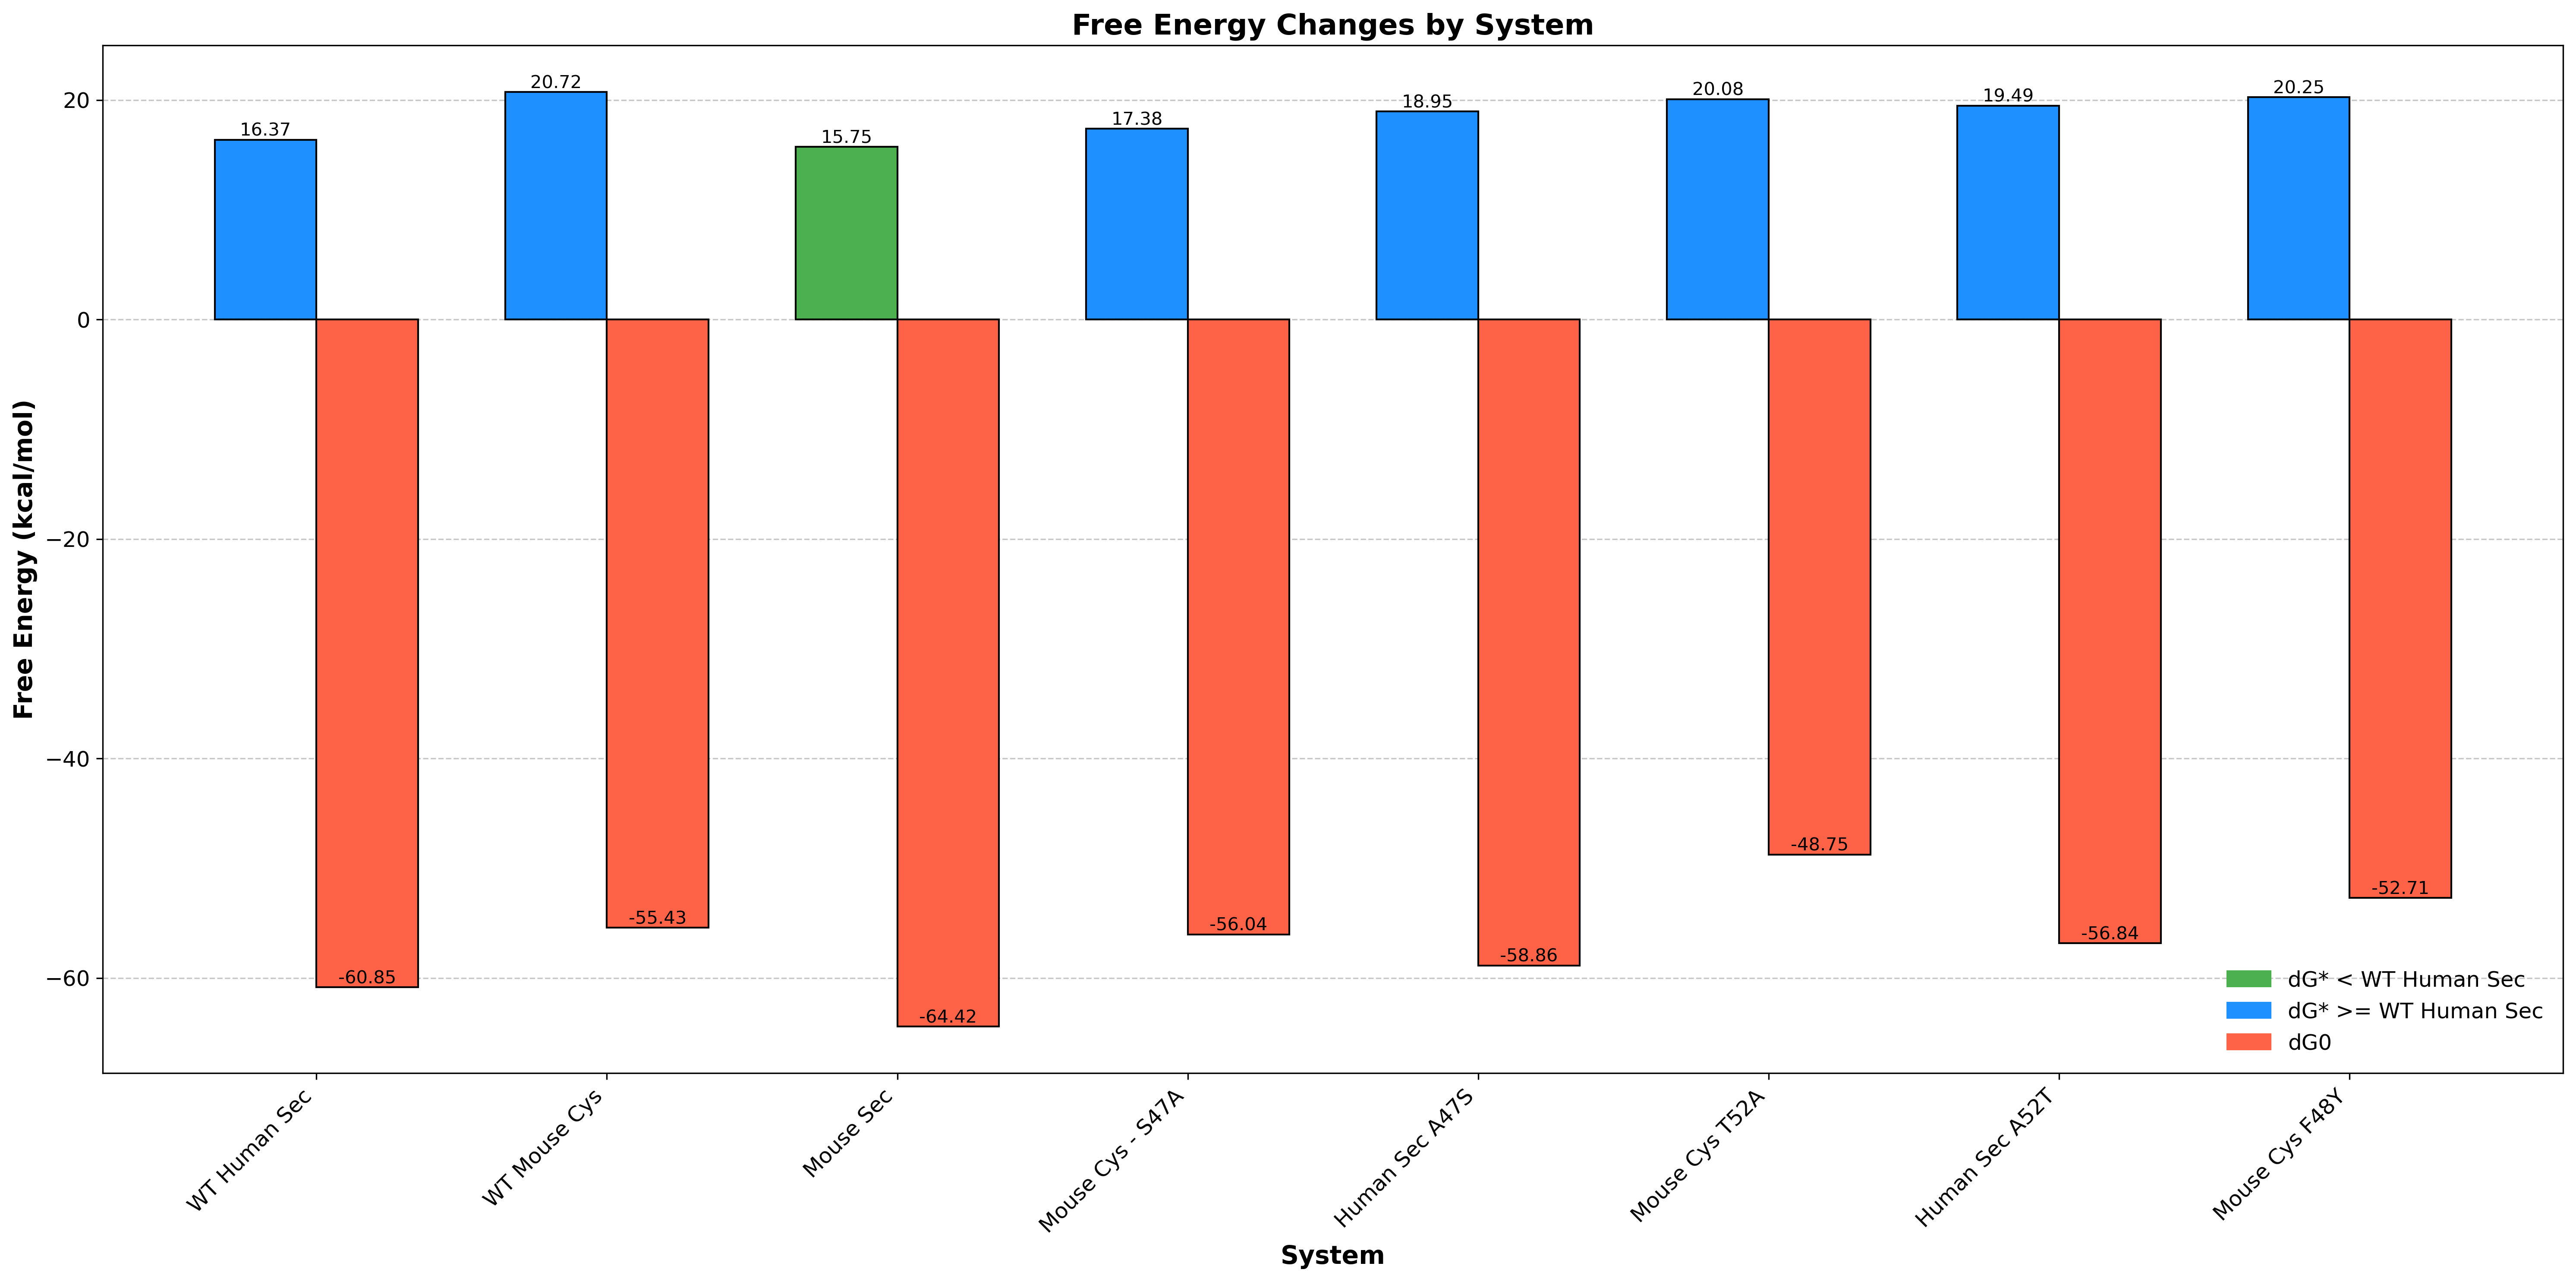
\includegraphics[width=\textwidth]{Free_Energy_BarPlot.png} % Ensure the path is correct
    \caption{Free Energy Bar Plot}
    \label{fig:free_energy_barplot}
\end{figure}

\end{document}
